\question[10] En la Figura \ref{fig:sucesion_triangulos01} se construye cada diseño con triángulos, añadiendo palillos de la
siguiente manera.

\begin{figure}[H]
    \centering
    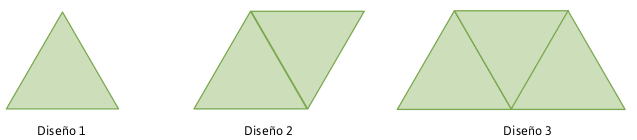
\includegraphics[width=.6\linewidth]{../images/sucesion_triangulos01}
    \caption{}
    \label{fig:sucesion_triangulos01}
\end{figure}

\begin{parts}
    \part Escribe una regla para la sucesión del número de palillos y compruébala.

    \begin{solutionbox}{1.2cm}
        $2n + 1$. En la comprobación se pueden incluir argumentos similares a
        los usados en los casos anteriores.
    \end{solutionbox}

    \part Calculen cuántos palillos se tienen en total en el diseño 19.

    \begin{solutionbox}{1.2cm}
        $2(19) + 1 = 39$.
    \end{solutionbox}

    \part Toma en cuenta las reglas $20 + n$ y $13 + 2(n - 6)$ y calculen su valor para n = 19.

    \begin{solutionbox}{1.6cm}
        Primera regla: $20 + (19) = 39$.\\
        Segunda regla: $13 + 2(19 - 6) = 13 + 2(13) = 13 + 26 = 39$.
    \end{solutionbox}

    \part Comparen los resultados de los incisos c) y d). ¿Cómo son? ¿Por qué?

    \begin{solutionbox}{1.2cm}
        Son iguales para n = 19.
    \end{solutionbox}

    \part Basados en los valores de la regla que cada uno encontró y de estas dos, ¿las ex-
    presiones son equivalentes? Expliquen.

    \begin{solutionbox}{2.4cm}
        La fórmula que describe la sucesión es equivalente a $13 + 2(n - 6)$,
        lo cual se demuestra simplifi cando la expresión de la siguiente manera:
        $13 + 2n - 12 = 2n + 1$.\\
        Sin embargo, la regla $20 + n$ sólo coincide con las otras para el valor $n = 19$.
        Por ejemplo, el primer término de la sucesión ($n = 1$) según esta fórmula, de-
        bería ser $20 + 1 = 21$, lo cual difiere de $2(1) + 1 = 3$.
    \end{solutionbox}

\end{parts}